\documentclass[]{report}

\usepackage{amsmath}
\usepackage{amssymb}
\usepackage{bm}
\usepackage{graphicx}
\usepackage{listings}

\graphicspath{ {images/} }

\title{CSCI 567 HW \# 5}
\author{Mohmmad Suhail Ansari \\ USC ID: 8518586692\\e-mail: mohmmada@usc.edu}

\begin{document}

\maketitle

\paragraph{Sol. 1.1}
	Given 
	\[ D = \sum_{n=1}^N \sum_{k=1}^K r_{nk}  {\| x_n - \mu_k \|}_2^2 \]
	taking partial derivative w.r.t. $\mu_k$, we get 
	\[ \frac{\partial{D}}{\partial{\mu_k}} = \sum_{n=1}^N r_{nk} [-2 (x_n - \mu_k)] = 0 \]
	\[ = \sum_{n=1}^N r_{nk} x_n - \mu_k \sum_{n=1}^N r_{nk} = 0\]
	\[ \mu_k = \frac{\sum_{n=1}^N r_{nk} x_n}{\sum_{n=1}^N r_{nk}}\]

\paragraph{Sol. 1.2}
	Given 
	\[ D = \sum_{n=1}^N \sum_{k=1}^K r_{nk}  {\| x_n - \mu_k \|}_1 \]
	We want find an optimal $\mu_k$, such that it minimizes $D$ and that optimal $\mu$ is equal to the 
	median of $x_n = [x_{n1}, x_{n2} \hdots x_{nD}]$.

	Now, let us assume that, $\mu_k$ is optimal and for a given vector $x_n, x_n \in R^D$, so fro the definition of 
	``closeness'' in the text we get that 
	\[ L = \sum_{i=1}^D |x_{ni} - \mu_k|\],
	Now if there are $l$ numbers to the left of $\mu_k$ and $r$ number to the right, then if we were to shift $\mu_k$ by a distance $d$
	to the left, the $L$ increases by $(l - r)d \quad if(l > r)$. Similarly if, we were to shift $\mu_k$ to the right by a distance of $d$, then again the 
	measurement of $L$ increases by $(r - l)d \quad if (r > l)$. Therefore $L$ will achieve if minimum value when $l = r$, i.e. $\mu_k$ is the median of the 
	vector $x_n$.


	Now we derive the above conclusion to multi-dimensionalities. We can see only when  is the elementwise median of cluster k, $L_k = \sum_{i=1}^{N_k} |x_i - \mu_k |$ has the minimal value. Suppose there are K clusters, the overall loss is
	\[ L = \sum_{k=1}^K L_k = \sum_{k=1}^K \sum_{n=1}^N |x_n - \mu_k| \]  
	which will also be minimal, which equals to 
	\[ D = \sum_{k=1}^K L_k = \sum_{k=1}^K \sum_{n=1}^N r_{nk} |x_n - \mu_k| \]  

\paragraph{Sol 1.3}
	Given
	\begin{equation}
		\tilde{D} = \sum_{n=1}^N \sum_{k=1}^K r_{nk} {\| \phi (x_n) - \tilde{\mu}_k \|}_2^2 
	\end{equation}

	where, 
	\begin{equation}
		\tilde{\mu}_k = \frac{1}{N_k} \sum_{n=1}^N r_{nk} \phi (x_n)
	\end{equation}

	We can write $\frac{r_{nk}}{N_k} = \gamma_{nk}$, then we can rewrite $\tilde{\mu}$ as 
	\[ \tilde{\mu}_k = \sum_{n=1}^N \gamma_{nk} \phi (x_n) \]
	
	Then, 
	\[ {\| \phi(x_n) - \tilde{\mu}\|}^2 = {\| \phi(x_n) - \sum_{n=1}^N \gamma_{nk} \phi (x_n) \|}^2 \]
	\[ = [\phi(x_n) - \sum_{n=1}^N \gamma_{nk} \phi (x_n)] \cdot [\phi(x_n) - \sum_{n=1}^N \gamma_{nk} \phi (x_n)] \]
	\[ = K(x, x) - 2 \sum_{i=1}^N \gamma_{ik} K(x, x_i) + \sum_{i=1}^N \sum_{j=1}^N \gamma_{ik} \gamma_{jk} K(x_i, x_j) \]

	Therefore, we can write
	\[ \tilde{D} = \sum_{n=1}^N \sum_{k=1}^K r_{nk} \big[ K(x_n, x_n) - 2 \sum_{i=1}^N \gamma_{ik} K(x_n, x_i) + \sum_{i=1}^N \sum_{j=1}^N \gamma_{ik} \gamma_{jk} K(x_i, x_j) \big] \]

	To assign a point to a cluster $k$, we initialize (randomly or through other methods) $\tilde{\mu}_k$ and for each iteration, assign, $x_n$ to k where
	\[ argmax_{k \in K} K(x_n, x_n) - 2 \sum_{i=1}^N \gamma_{ik} K(x_n, x_i) + \sum_{i=1}^N \sum_{j=1}^N \gamma_{ik} \gamma_{jk} K(x_i, x_j) \]

	The pseudo-code 
	\newpage

\begin{lstlisting}
Kernel_Kmeans():
  G = GramMatrix(X)
  Assignment = init_random_assigmnment()
  Means = random.sample(X, k)
  for max_iterations:
  	for k in K:
  	  for i, x in enumerate(X):
	        distance[i, k] =  G[x, x] 
	        distance[i, k] -= (2 * sum(G[(Assignment == k), i]) 
	        distance[i, k] += sum(G[Assignment == k, Assignment == k]) 
    Assignment = argmin(distance)
    for k in K:
      NewMeans[k] = mean(X[Assignment == k])
    if convereged(Means, NewMeans):
      return Assignment, NewMeans
    else:
      Means = NewMeans
\end{lstlisting}


\paragraph{Sol 2.1}
	We can write the likelihood function as 
	\[ p(x | \alpha) = \frac{\alpha}{\sqrt{2 \pi}} exp(-\frac{1}{2} x^2) + \frac{1 - \alpha}{\sqrt{\pi}} exp(- x^2)\]
	and for observed sample $x_1$, we can write
	\[ p(x_1 | \alpha) = (\frac{1}{\sqrt{2 \pi}} exp(-\frac{1}{2}x_1^2) - \frac{1}{\sqrt(\pi)} exp(-x_1^2)) \alpha + \frac{1}{\sqrt{\pi}} exp(-x^2) \]
	We observe the likelihood function for an observed sample $x_1$ is a linear function of $\alpha$ where the slope of the line is determined by the values of the gaussian probabilities. So, for maximum likelihood, if the gaussian probability $N(x_1 | 0, 1) > N(x_1|0, 0.5)$ then we choose $\alpha = 1$ for maximum likelihood, else we choose $\alpha = 0$.

\paragraph{Sol 3.1}
	Let us define the hidden variable as $z_i = 1$ when a person in the sample has taken insurance, and $z_i = 0$ otherwise. Now, if $x_i > 0$, then clearly $z_i = 1$, however, when $x_i = 0$, then $z_i = 1$ or $0$.

	Therefore our likelihood function can be given as 
	\[ 
		L = \prod_{i=1}^N \pi^{1-u_i} \big[ (1 - \pi) \frac{e^{-\lambda} \lambda^{x_i}}{x_i!} \big]^{u_i}
	\]

	where $u_i = 1$ if $x_i > 0$ and $u_i = z_i$ if $x_i = 0$.

\paragraph{Sol 3.2} N/A


\paragraph{Sol 4.1}
	\begin{center}
		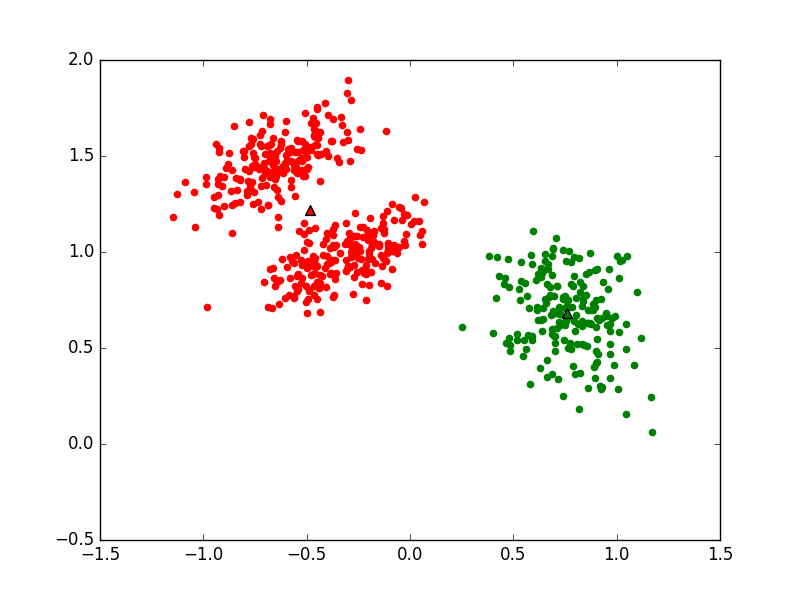
\includegraphics[width=\textwidth]{blob-2}
		Blob, K = 2
		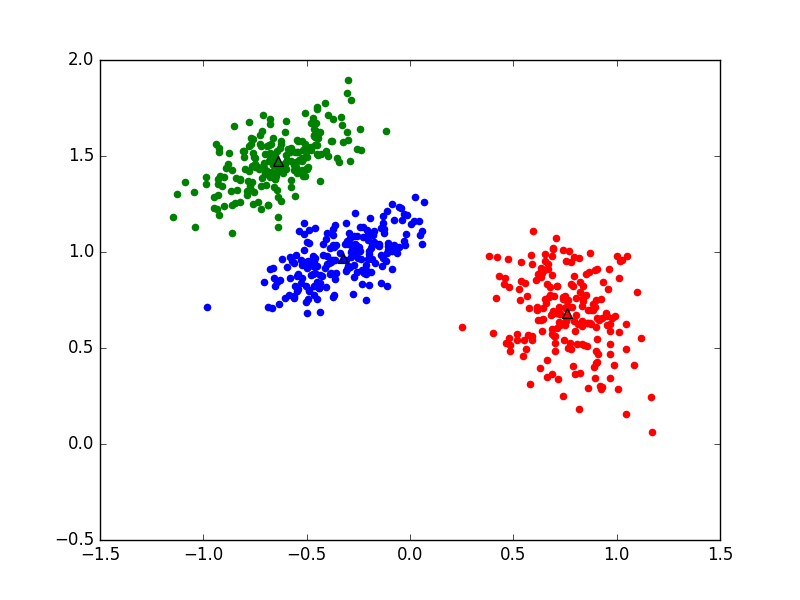
\includegraphics[width=\textwidth]{blob-3}
		Blob, K = 3
		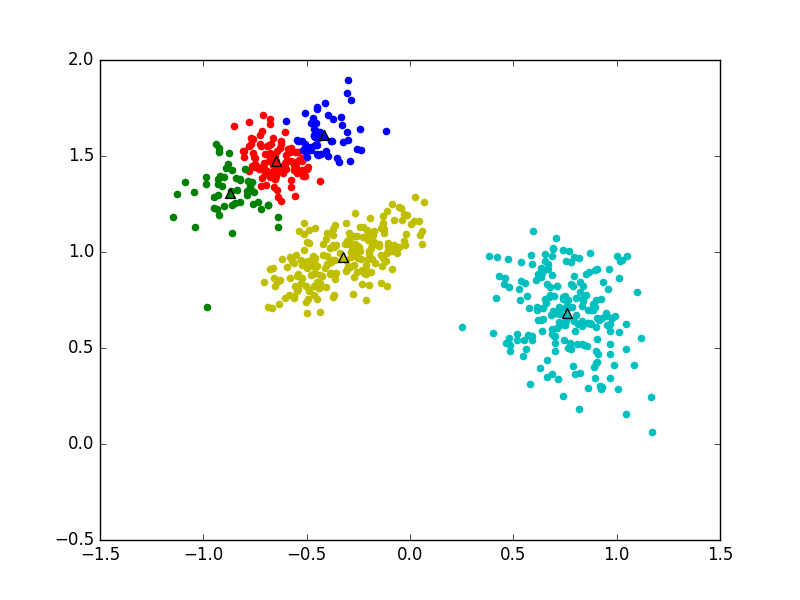
\includegraphics[width=\textwidth]{blob-5}
		Blob, K = 5
		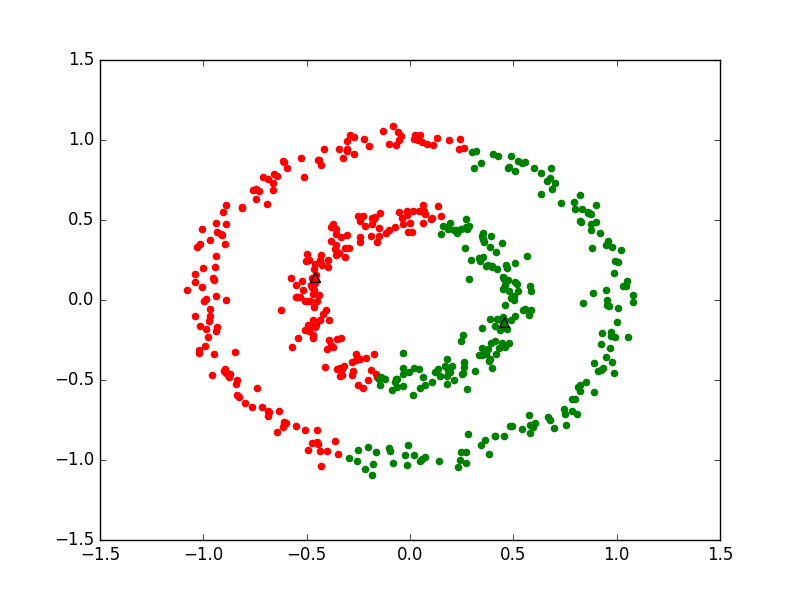
\includegraphics[width=\textwidth]{circle-2}
		Circle, K = 2
		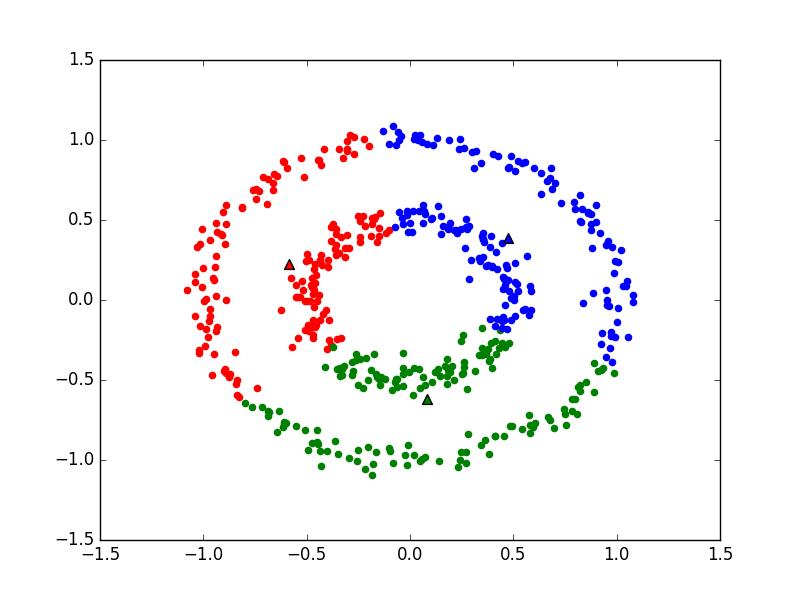
\includegraphics[width=\textwidth]{circle-3}
		Circle, K = 3
		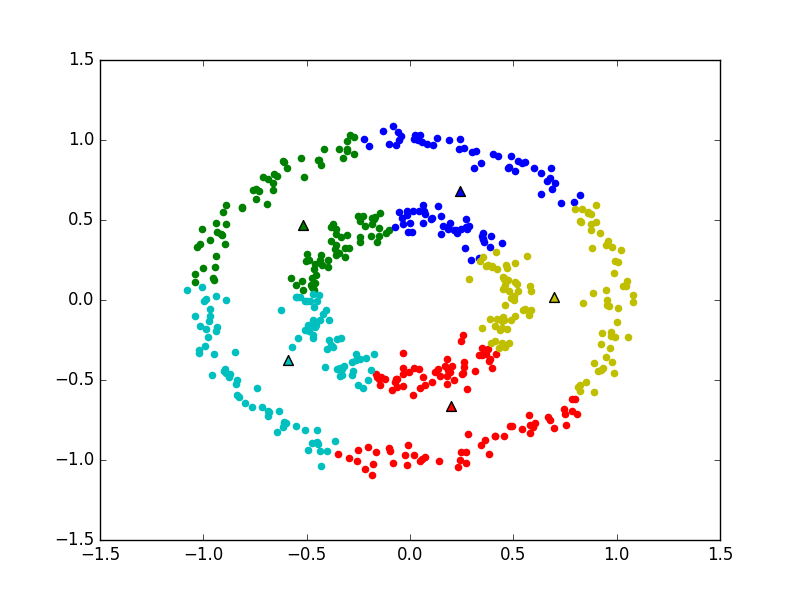
\includegraphics[width=\textwidth]{circle-5}
		Circle, K = 5
	\end{center}

	For $\texttt{circle.csv}$ and $K = 2$, since, both the clusters are concentric circles and their centroid falls at the same point and hence for a point the difference between minimum distances is small or equal.

\paragraph{Sol 4.2}
	Using the feature transformation
	\[ \phi(x, y) = [x, y, 2(x^2 + y^2)] \]
	
	\begin{center}
		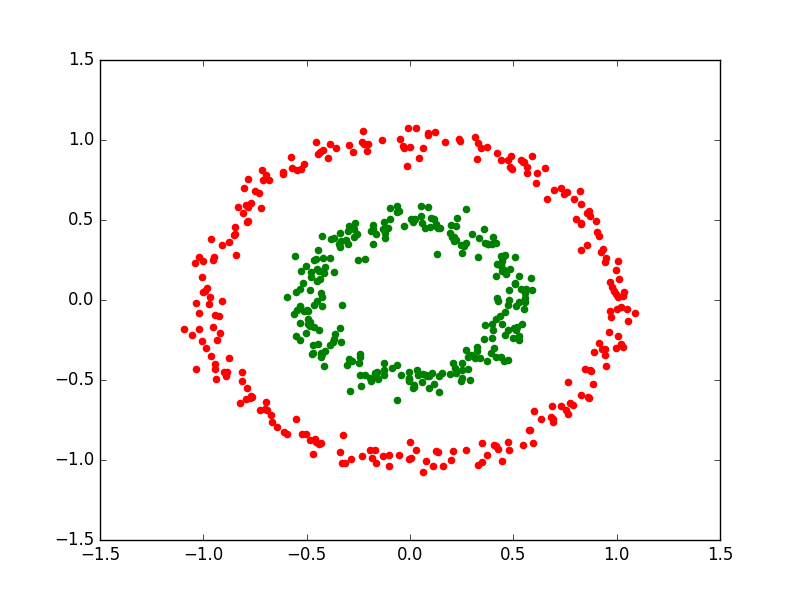
\includegraphics[width=\textwidth]{Kernel-Kmeans-2}
		k = 2
	\end{center}

\paragraph{Sol 4.3}

	\begin{center}
		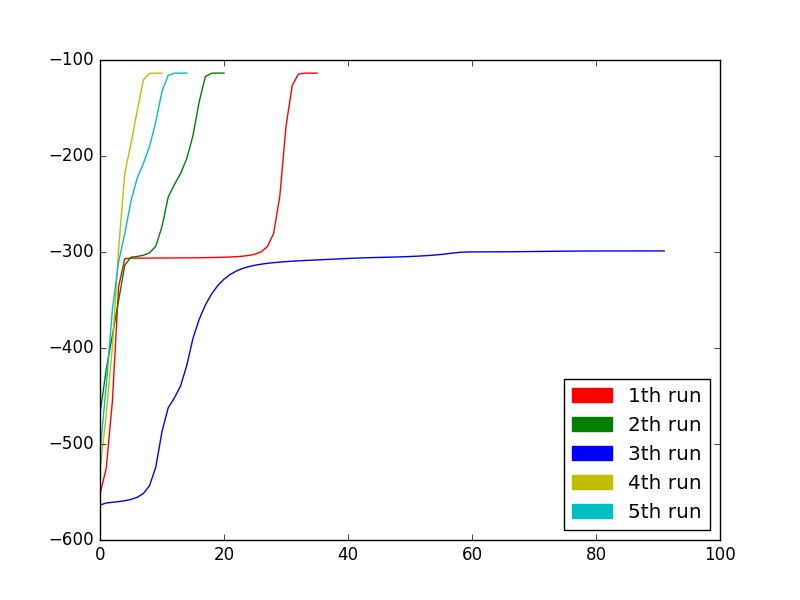
\includegraphics[width=\textwidth]{LogLikelihood}
		Log-Likehood Plot
		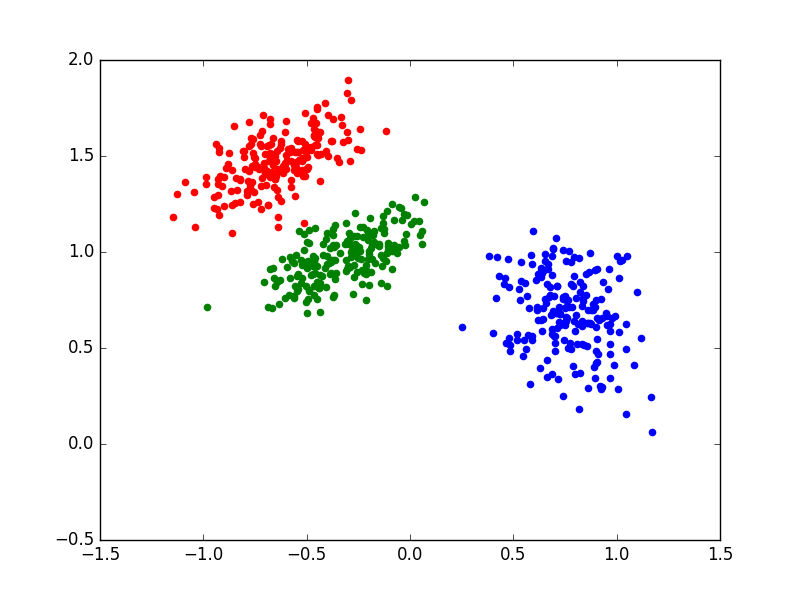
\includegraphics[width=\textwidth]{EM-Scatterplot}
		Cluster Assignment Plot
	\end{center}
\[ 
	Means = \begin{bmatrix}
		K=1 &   0.75896032 & 0.67976983 \\
		K=2 &  -0.32591595 & 0.97133268 \\
		K=3 &  -0.63946222 & 1.47460006 
	\end{bmatrix} 
\]

\[
	Covariance[k = 1] = \begin{bmatrix}
		0.02717056  & -0.00840045 \\
	 	-0.00840045 &  0.040442 
	\end{bmatrix}
\]
\[	
	Covariance[k = 2] = \begin{bmatrix}
		0.03604869 & 0.01463998 \\
 		0.01463998 & 0.01629099 
	\end{bmatrix}
\]
\[	
	Covariance[k = 3] = \begin{bmatrix}
		0.03596703 & 0.01549264  \\
 		0.01549264 & 0.01935347 
	\end{bmatrix}
\]

\end{document}